\section{Ramas de la IA Aplicadas a la Industria}\label{ramas-de-la-ia-aplicadas-a-la-industria}

\begin{figure}[H]
\centering
\begin{adjustbox}{width=\textwidth}
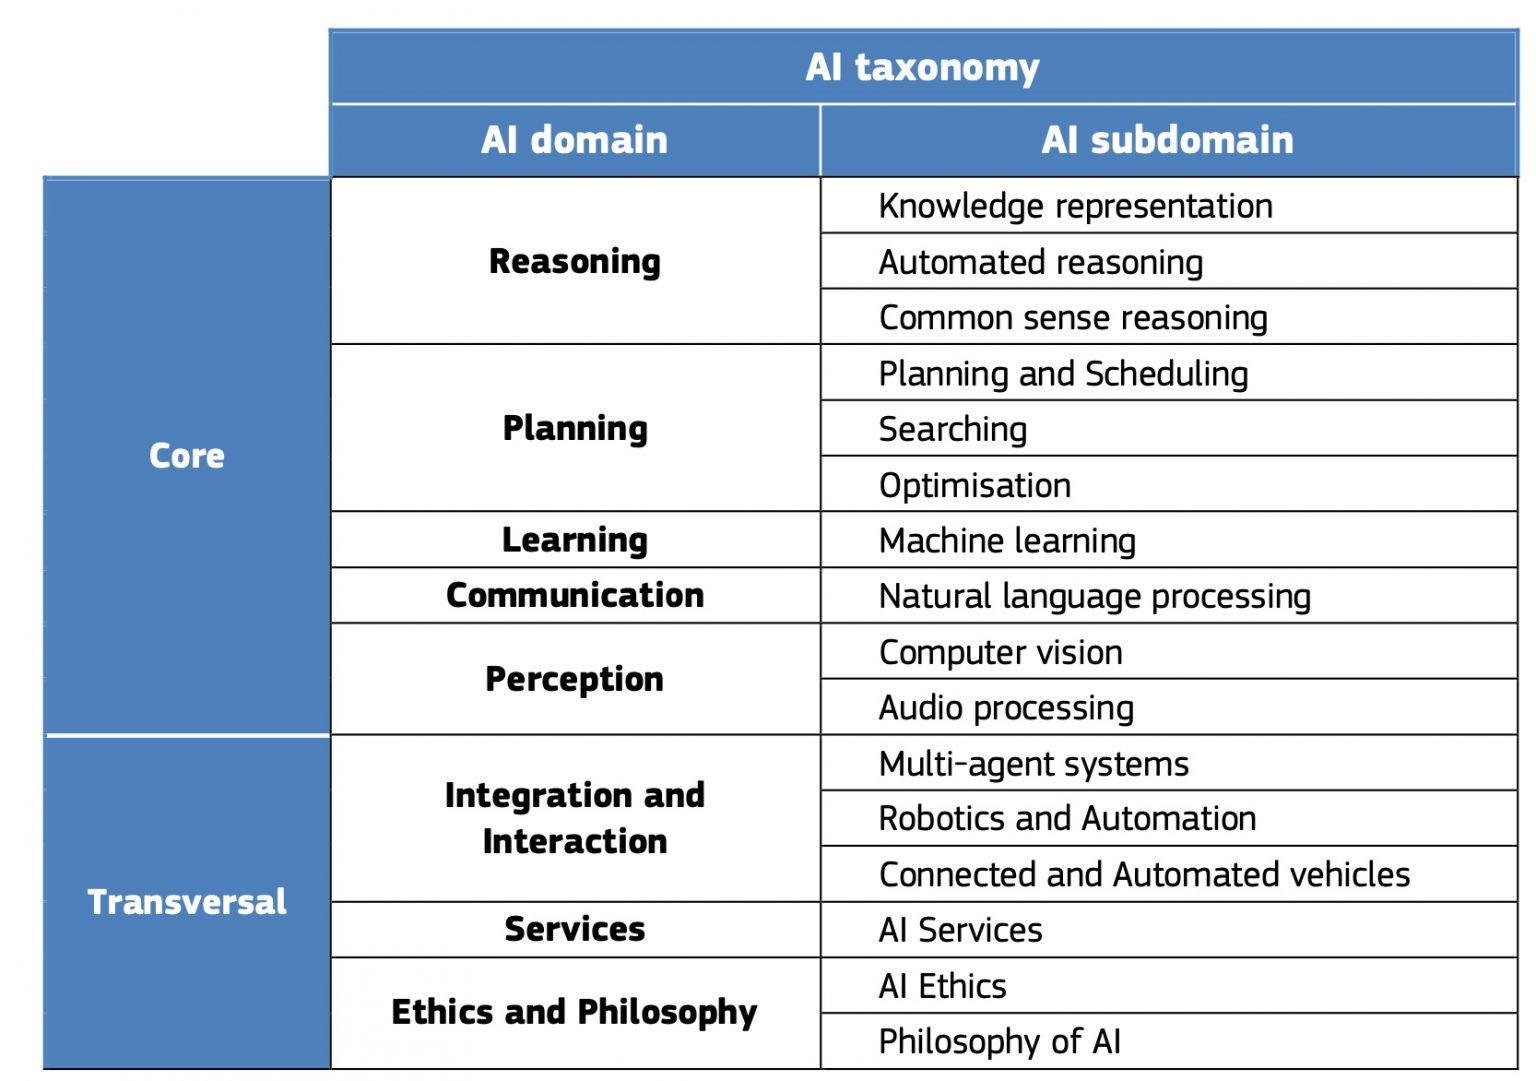
\includegraphics{img/taxonomia.jpg}
\end{adjustbox}
\caption{Taxonomía de la IA aplicada a la industria}
\label{fig:taxonomia-ia}
\end{figure}

Esta imagen presenta una \textbf{taxonomía de la Inteligencia Artificial (IA)}, organizada en dominios y subdominios, que abarca tanto aspectos \textbf{centrales (Core)} como \textbf{transversales (Transversal)} de la IA. Aquí te explico cada sección:

\subsection{Dominio Central (Core)}\label{dominio-central-core}
Estos son los fundamentos o los componentes clave de la IA, que abarcan desde cómo razona una máquina hasta cómo percibe e interactúa con el mundo.

\begin{enumerate}
\item \textbf{Reasoning (Razonamiento)}
  \begin{itemize}
    \item \textbf{Knowledge Representation}: Representación del conocimiento. Se refiere a cómo una máquina organiza y almacena la información de manera que pueda usarla para tomar decisiones o resolver problemas.
    \item \textbf{Automated Reasoning}: Razonamiento automatizado. La capacidad de la IA para derivar conclusiones y resolver problemas complejos basados en las reglas y el conocimiento almacenado.
    \item \textbf{Common Sense Reasoning}: Razonamiento de sentido común. La IA intenta razonar como lo haría una persona, utilizando conocimientos que los humanos damos por sentado, pero que las máquinas deben aprender o codificar.
  \end{itemize}

\item \textbf{Planning (Planificación)}
  \begin{itemize}
    \item \textbf{Planning and Scheduling}: Planificación y programación. La capacidad de la IA para organizar tareas o recursos en función de objetivos, optimizando tiempos y recursos.
    \item \textbf{Searching}: Búsqueda. IA encuentra soluciones a problemas o información relevante entre un conjunto de opciones.
    \item \textbf{Optimisation}: Optimización. Aquí la IA busca la mejor solución entre múltiples alternativas, ajustando variables para obtener el mejor rendimiento o eficiencia.
  \end{itemize}

\item \textbf{Learning (Aprendizaje)}
  \begin{itemize}
    \item \textbf{Machine Learning}: Aprendizaje automático. Esta es la capacidad de las máquinas para aprender a partir de datos sin ser programadas explícitamente para cada tarea. Es una de las áreas más destacadas y utilizadas en la IA actual.
  \end{itemize}

\item \textbf{Communication (Comunicación)}
  \begin{itemize}
    \item \textbf{Natural Language Processing}: Procesamiento del lenguaje natural. La IA comprende, interpreta y genera lenguaje humano, facilitando la interacción entre humanos y máquinas mediante el habla o el texto.
  \end{itemize}

\item \textbf{Perception (Percepción)}
  \begin{itemize}
    \item \textbf{Computer Vision}: Visión por computadora. La IA percibe el mundo visualmente, analizando imágenes o videos para detectar patrones, objetos o reconocer caras.
    \item \textbf{Audio Processing}: Procesamiento de audio. Similar a la visión por computadora, pero en este caso, la IA procesa y entiende sonidos, como la voz o música.
  \end{itemize}
\end{enumerate}

\subsection{Dominio Transversal}\label{dominio-transversal}

Estas áreas complementan los dominios centrales, ofreciendo integración, interacción y aspectos filosóficos o éticos.

\begin{enumerate}
\item \textbf{Integration and Interaction (Integración e Interacción)}
  \begin{itemize}
    \item \textbf{Multi-agent Systems}: Sistemas multiagente. Conjunto de IA que trabajan juntas, colaborando o compitiendo para resolver problemas más complejos.
    \item \textbf{Robotics and Automation}: Robótica y automatización. Integra la IA con robots y sistemas automatizados para realizar tareas físicas, como ensamblar productos en fábricas.
    \item \textbf{Connected and Automated Vehicles}: Vehículos conectados y automatizados. Implica el uso de IA para controlar vehículos autónomos y conectados que operan sin intervención humana.
  \end{itemize}

\item \textbf{Services (Servicios)}
  \begin{itemize}
    \item \textbf{AI Services}: Servicios de IA. Herramientas y plataformas basadas en IA que las empresas y personas pueden utilizar para resolver problemas o mejorar procesos (por ejemplo, asistentes virtuales, análisis predictivos).
  \end{itemize}

\item \textbf{Ethics and Philosophy (Ética y Filosofía)}
  \begin{itemize}
    \item \textbf{AI Ethics}: Ética de la IA. Se ocupa de las cuestiones éticas relacionadas con el uso y el desarrollo de la IA, como la privacidad, la equidad y el impacto social.
    \item \textbf{Philosophy of AI}: Filosofía de la IA. Reflexiones más profundas sobre el papel de la IA en la sociedad y qué significa para las máquinas tener inteligencia similar a la humana.
  \end{itemize}
\end{enumerate}

\subsection{Resumen}\label{resumen}

La taxonomía de la IA presentada en esta imagen divide los conceptos fundamentales en dominios que abarcan \textbf{razonamiento}, \textbf{planificación}, \textbf{aprendizaje}, \textbf{comunicación} y \textbf{percepción}. Estos conceptos son claves para entender cómo la IA interactúa y aprende del mundo. Los dominios transversales complementan estas capacidades con aspectos como la \textbf{integración}, los \textbf{servicios de IA} y las \textbf{cuestiones éticas}, que son fundamentales para asegurar un uso responsable y eficaz de la inteligencia artificial en el mundo real.


\section{IA Simbólica}\label{ia-simbolica}

La Inteligencia Artificial Simbólica es un enfoque de la IA que se basa en representar el conocimiento y el razonamiento a través de símbolos y reglas lógicas. En lugar de aprender a partir de datos, como ocurre en el Machine Learning, la IA simbólica funciona siguiendo un conjunto de instrucciones predefinidas para resolver problemas o tomar decisiones.

Por ejemplo, en una maquiladora donde se ensamblan componentes electrónicos, la IA simbólica puede controlar la temperatura de las máquinas o la calidad de los productos sin margen de error, gracias a sus reglas fijas. Este enfoque es ideal para tareas donde no hay mucha variabilidad, y se requiere cumplir con estrictos parámetros de producción.

Este enfoque es como una receta: todo está previamente determinado, y la máquina sigue los pasos sin desviarse. Un sistema de IA simbólica podría estar programado para diagnosticar fallos en una máquina si ciertas condiciones, como la temperatura o la vibración, exceden los límites establecidos. Cada condición está claramente definida, y la IA actúa según las reglas sin necesidad de adaptarse o aprender nuevas formas de solucionar el problema.

La IA Simbólica es particularmente útil en entornos donde los procesos son repetitivos o bien estructurados. Aunque no es flexible como el Machine Learning, la IA simbólica es extremadamente precisa y eficiente cuando se trata de ejecutar tareas que siguen un patrón fijo y bien entendido.

\subsection{Ejemplo: IA Simbólica con Receta de Cocina}\label{ejemplo-ia-simbolica}

\textbf{Imagina} que le das a un robot una receta detallada para hacer un pastel. Le das instrucciones específicas como:

\begin{enumerate}
    \item Mezcla 200 gramos de harina con 100 gramos de azúcar.
    \item Añade dos huevos y bate la mezcla por 5 minutos.
    \item Coloca la mezcla en el horno a 180°C durante 30 minutos.
\end{enumerate}

Este tipo de robot es un ejemplo de \textbf{IA Simbólica}, porque sigue un conjunto de reglas claras para completar la tarea. Cada paso está definido de manera precisa, y el robot simplemente sigue las instrucciones. Si la receta no cambia, el robot siempre hará el pastel de la misma manera, una y otra vez.

\subsection{Ejemplo: Machine Learning como Chef Aprendiz}\label{ejemplo-machine-learning}

Ahora, \textbf{imagina} que en lugar de seguir siempre la misma receta, tienes un robot que quiere convertirse en un chef experto. En lugar de seguir instrucciones precisas, este robot observa a diferentes cocineros haciendo pasteles y aprende de sus técnicas. Tal vez nota que algunos cocineros usan más azúcar, otros agregan ingredientes extra como vainilla, y algunos hornean el pastel por más tiempo dependiendo del tipo de horno. El robot comienza a \textbf{aprender} que, dependiendo de ciertos factores, puede ajustar la receta para hacer el mejor pastel posible.

Este es un ejemplo de \textbf{Machine Learning}, donde la IA no sigue reglas predefinidas, sino que aprende a partir de los datos que recopila. En lugar de seguir la misma receta siempre, el robot adapta la receta según los datos que ha recopilado.

\subsection{Comparando los Enfoques}\label{comparacion-enfoques}

\begin{itemize}
    \item \textbf{IA Simbólica}: Es como el robot que sigue una receta fija. Funciona bien en situaciones donde las reglas son claras y no cambian mucho. Esto es útil en procesos repetitivos como el ensamblaje en una maquila, donde los pasos son los mismos cada día.
    \item \textbf{Machine Learning}: Es como el chef aprendiz. En lugar de seguir reglas fijas, aprende y mejora con el tiempo a medida que recopila más información.
\end{itemize}

\subsection{Ejemplo: IA en el Control de Calidad}\label{ejemplo-control-calidad}

\textbf{Imagina} que en tu maquila produces miles de piezas cada día, y necesitas asegurarte de que todas cumplan con los estándares de calidad. En lugar de tener a una persona revisando cada pieza (lo cual puede ser lento y propenso a errores), podrías usar \textbf{IA Simbólica} o \textbf{Machine Learning}.

\begin{itemize}
    \item Con \textbf{IA Simbólica}, podrías programar una máquina para revisar cada pieza siguiendo reglas específicas. Por ejemplo: ``Si la pieza tiene más de 0.5 mm de desviación, recházala''. Esto es eficiente, pero solo funciona para detectar errores simples.
    \item Con \textbf{Machine Learning}, podrías entrenar una máquina para detectar patrones más complejos. El sistema podría aprender a reconocer qué tipo de defectos aparecen con mayor frecuencia y, con el tiempo, predecir dónde y cuándo es más probable que aparezcan defectos, ajustando la producción en consecuencia. Podría incluso aprender de nuevos datos para mejorar la precisión a lo largo del tiempo.
\end{itemize}

\subsection{Reflexión Final: Bajar la IA a lo Práctico}\label{reflexion-practica}

La IA, en su forma más simple, es una herramienta que ayuda a las máquinas a hacer tareas que normalmente haría un humano, pero con mayor precisión y eficiencia. No necesitas ser un experto para empezar a entender cómo puede mejorar tu maquila. Lo importante es reconocer que hay dos formas principales en que la IA puede ayudarte: \textbf{siguiendo reglas fijas (IA Simbólica)} o \textbf{aprendiendo de los datos (Machine Learning)}. Y aunque los conceptos técnicos puedan sonar complicados, los beneficios prácticos son claros: más eficiencia, menos errores, y una producción más ágil y adaptada a las necesidades del día a día.

\section{Perfil para Trabajar con IA Simbólica en una Maquiladora}\label{perfil-ia-simbolica}

Para implementar y gestionar la \textbf{IA Simbólica} en una maquiladora, se necesita un perfil multidisciplinario que combine habilidades técnicas con un profundo conocimiento de los procesos industriales. A continuación, te describo el perfil ideal para alguien que trabajará en la adopción y gestión de la IA simbólica en un entorno de producción.

\subsection{Conocimiento Técnico en Programación y Lógica}

Dado que la IA simbólica se basa en reglas predefinidas y condiciones lógicas, es crucial que el candidato tenga sólidos conocimientos de \textbf{programación} y \textbf{lógica de procesos}. Estos son algunos de los requisitos técnicos:

\begin{itemize}
    \item \textbf{Lenguajes de Programación}: Competencia en lenguajes de programación que permiten definir reglas y algoritmos, como \textbf{Python}, \textbf{C++}, o lenguajes específicos de automatización industrial (como \textbf{Ladder Logic} o \textbf{Structured Text} para PLCs).
    \item \textbf{Experiencia en Sistemas de Automatización}: Conocimiento de sistemas SCADA o PLC (Controladores Lógicos Programables) que se utilizan ampliamente en entornos industriales.
    \item \textbf{Manejo de Reglas Lógicas}: Habilidad para diseñar y gestionar reglas de ``si-entonces'' (if-then) y otros tipos de reglas lógicas que determinan el comportamiento de los sistemas de IA simbólica.
    \item \textbf{Diagramas de Flujo}: Capacidad para diseñar, interpretar y modificar diagramas de flujo que describen el funcionamiento del sistema de IA simbólica.
\end{itemize}

\subsection{Conocimiento en Procesos Industriales}

Es fundamental que la persona tenga un buen entendimiento de los procesos específicos de la \textbf{industria maquiladora}. Esto permitirá al profesional identificar las áreas donde la IA simbólica puede ser más útil y generar un mayor impacto en la eficiencia y automatización de procesos.

\begin{itemize}
    \item \textbf{Control de Calidad}: Comprender cómo funcionan los sistemas de control de calidad en la línea de producción y cómo la IA puede optimizar el proceso mediante reglas predefinidas para la detección de defectos.
    \item \textbf{Gestión de Inventarios}: Saber cómo operan los sistemas de inventario y cómo las reglas lógicas pueden automatizar las órdenes de compra y el reabastecimiento.
    \item \textbf{Mantenimiento de Máquinas}: Conocimiento sobre los ciclos de mantenimiento y cómo establecer reglas simbólicas para alertas y paradas preventivas.
\end{itemize}

\subsection{Habilidad para Diseñar Sistemas Basados en Reglas}

Una de las tareas más importantes de este perfil es diseñar y optimizar las reglas que seguirá la IA simbólica. Esto requiere una capacidad para crear reglas claras y efectivas que cubran todas las posibles condiciones y escenarios que pueden presentarse en la maquiladora.

\begin{itemize}
    \item \textbf{Diseño de Reglas Condicionales}: Capacidad para desarrollar un sistema de reglas eficiente, asegurándose de que todas las situaciones posibles estén cubiertas. Ejemplo: ``Si el nivel de vibración de una máquina supera el umbral X, entonces enviar una alerta.''
    \item \textbf{Optimización de Procesos}: Habilidad para analizar y optimizar procesos mediante la creación de flujos lógicos claros, reduciendo tiempos muertos y aumentando la eficiencia de la producción.
\end{itemize}

\subsection{Experiencia en Implementación de Soluciones de IA Simbólica}

El candidato debe tener experiencia práctica en la implementación de sistemas basados en IA simbólica, desde el diseño inicial hasta la puesta en marcha y ajuste de reglas en entornos reales de producción.

\begin{itemize}
    \item \textbf{Configuración e Integración}: Capacidad para configurar la IA simbólica en los sistemas existentes, integrando la tecnología con otras soluciones industriales como ERPs, SCADA, o sistemas de gestión de inventarios.
    \item \textbf{Pruebas y Validación}: Habilidad para realizar pruebas y validar que las reglas y condiciones están funcionando de acuerdo con lo esperado, ajustando según sea necesario para mejorar la precisión del sistema.
\end{itemize}

\section{Ejemplo Práctico: Sistema de Control de Inventario}\label{ejemplo-control-inventario}

Imagina que en tu maquiladora manejas grandes cantidades de inventario y necesitas automatizar el proceso de reabastecimiento. Tradicionalmente, un encargado del almacén revisa manualmente los niveles de stock y crea órdenes de compra cuando se está quedando sin material. Este proceso manual puede ser ineficiente, propenso a errores y muy dependiente de una sola persona.

Al implementar un sistema basado en \textbf{IA Simbólica}, puedes automatizar este proceso completamente, eliminando la necesidad de revisiones manuales y reduciendo la dependencia del personal para mantener los niveles de stock óptimos. El sistema analizaría continuamente los niveles de inventario y generaría órdenes de compra automáticamente cuando sea necesario.

\subsection{Dataset de Ejemplo para Mantenimiento Predictivo}\label{dataset-mantenimiento-predictivo}

Además de optimizar el inventario, la IA también puede utilizarse para el mantenimiento predictivo de las máquinas. A continuación, se muestra un ejemplo de un dataset que podría usarse para entrenar un modelo de Machine Learning que prediga cuándo es probable que una máquina falle o necesite mantenimiento:

\begin{table}[htbp]
\centering
\begin{tabular}{|c|c|c|c|c|}
\hline
ID Máquina & Temperatura & Horas de Operación & Tipo de Máquina & Mantenimiento Urgente \\
\hline
1 & 85°C & 200 & Soldadora & Sí \\
2 & 70°C & 300 & Ensambladora & No \\
3 & 90°C & 180 & Cortadora & Sí \\
\hline
\end{tabular}
\caption{Ejemplo de dataset de mantenimiento predictivo en maquiladoras}
\label{tab:mantenimiento-predictivo}
\end{table}

Este dataset puede ser usado para entrenar un modelo de Machine Learning que prediga si una máquina va a necesitar mantenimiento en el futuro. El modelo analizaría las variables (temperatura, horas de operación, tipo de máquina) para predecir cuándo será necesario el mantenimiento, permitiendo que las intervenciones sean más proactivas en lugar de reactivas.

\subsection{Diagrama de Flujo para IA Simbólica}\label{diagrama-flujo}

Un diagrama de flujo es una representación gráfica de un proceso. En el caso de la IA simbólica, se puede utilizar para ilustrar cómo las reglas lógicas guían el comportamiento del sistema. Estas reglas definen un conjunto claro de condiciones, y el sistema actúa automáticamente dependiendo de si se cumplen o no.

\begin{figure}[H]
\centering
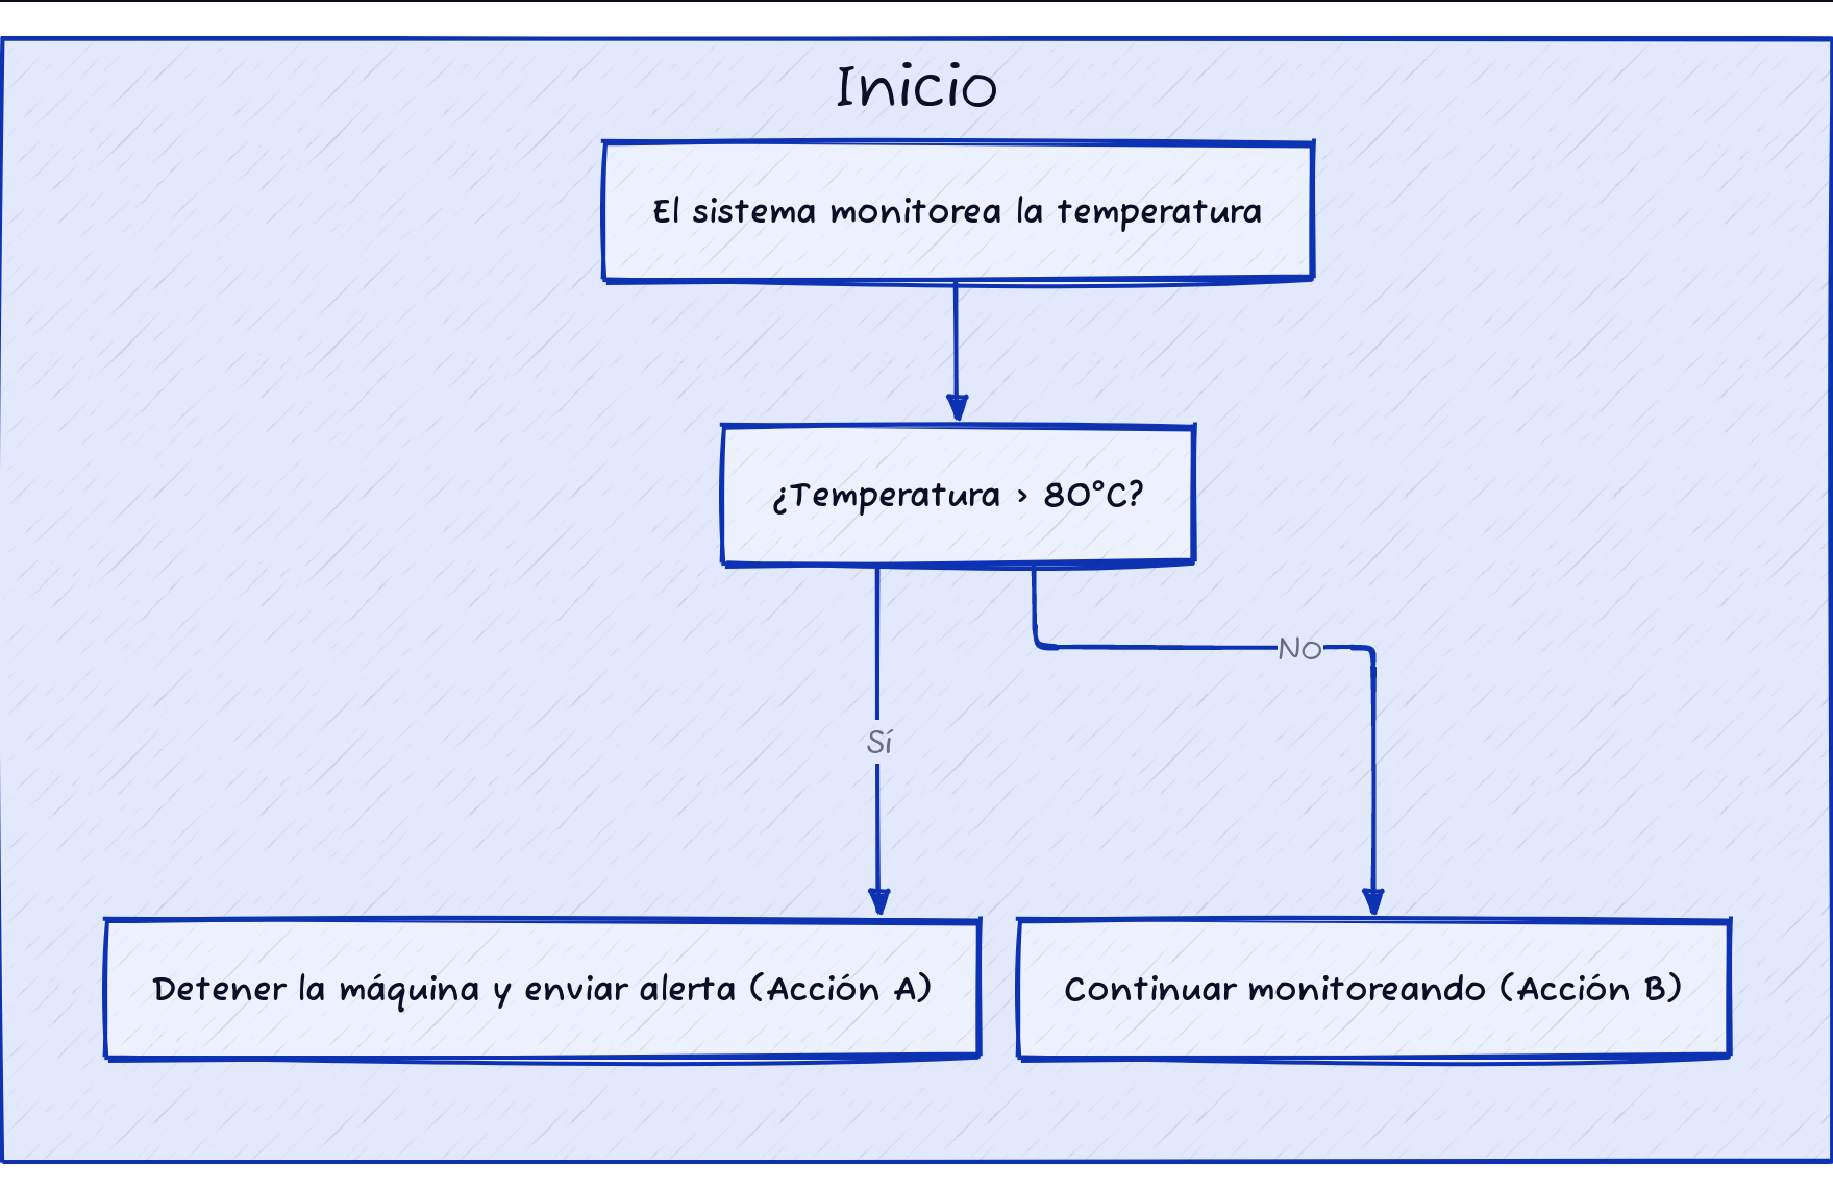
\includegraphics[h!,scale=0.5]{pdfs/diagram-1.pdf} 
\caption{Diagrama de flujo para IA simbólica en un sistema de inventario}
\label{fig:diagrama-flujo}
\end{figure}

En este flujo, cada decisión está basada en una condición clara que lleva a una acción específica. Esto es exactamente cómo funciona la IA simbólica: sigue reglas predefinidas sin necesidad de aprender o ajustarse con el tiempo. Por ejemplo:

\begin{itemize}
    \item \textbf{Condición 1:} Si el nivel de stock de un producto es menor a 50 unidades, enviar una alerta.
    \item \textbf{Condición 2:} Si el nivel de stock es menor a 10 unidades, generar automáticamente una orden de compra.
\end{itemize}

Este tipo de lógica reduce significativamente la intervención manual, permitiendo que el sistema mantenga el inventario de manera eficiente y asegurando que nunca haya falta de material para la producción.

\subsection{Implementación de un Sistema de Control de Inventario Basado en IA Simbólica}\label{implementacion-control-inventario}

Para implementar un sistema de control de inventario basado en \textbf{IA Simbólica}, los siguientes pasos serían esenciales:

\begin{enumerate}
    \item \textbf{Identificación de Variables Críticas:} El primer paso es identificar qué variables son clave para el proceso de control de inventario. Esto puede incluir el nivel de stock actual, la demanda histórica del producto, y el tiempo de reabastecimiento de los proveedores.
    
    \item \textbf{Definición de Reglas de Negocio:} Una vez identificadas las variables críticas, se deben definir las reglas de negocio que el sistema seguirá. Por ejemplo, \textit{"Si el nivel de stock de un producto es menor a 50 unidades, generar una alerta"}.
    
    \item \textbf{Automatización de Decisiones:} El sistema debe ser capaz de tomar decisiones automáticas basadas en estas reglas de negocio. Esto incluye la generación automática de órdenes de compra cuando los niveles de stock caigan por debajo de un umbral predefinido.
    
    \item \textbf{Monitoreo y Ajuste del Sistema:} Una vez que el sistema esté en funcionamiento, es importante monitorear su desempeño y realizar ajustes según sea necesario. Esto puede incluir la modificación de las reglas o la incorporación de nuevas variables.
\end{enumerate}

El beneficio de este tipo de sistema es que es extremadamente preciso y elimina el riesgo de errores humanos. Además, reduce la necesidad de intervención manual en procesos que de otro modo serían tediosos y propensos a errores.

\subsection{Diagrama de Flujo Extendido para IA Simbólica}\label{diagrama-flujo-extendido}

En un sistema más complejo, la IA simbólica puede manejar múltiples condiciones y tomar decisiones en función de diversos factores, como se muestra en el siguiente diagrama de flujo:

\begin{figure}[H]
\centering
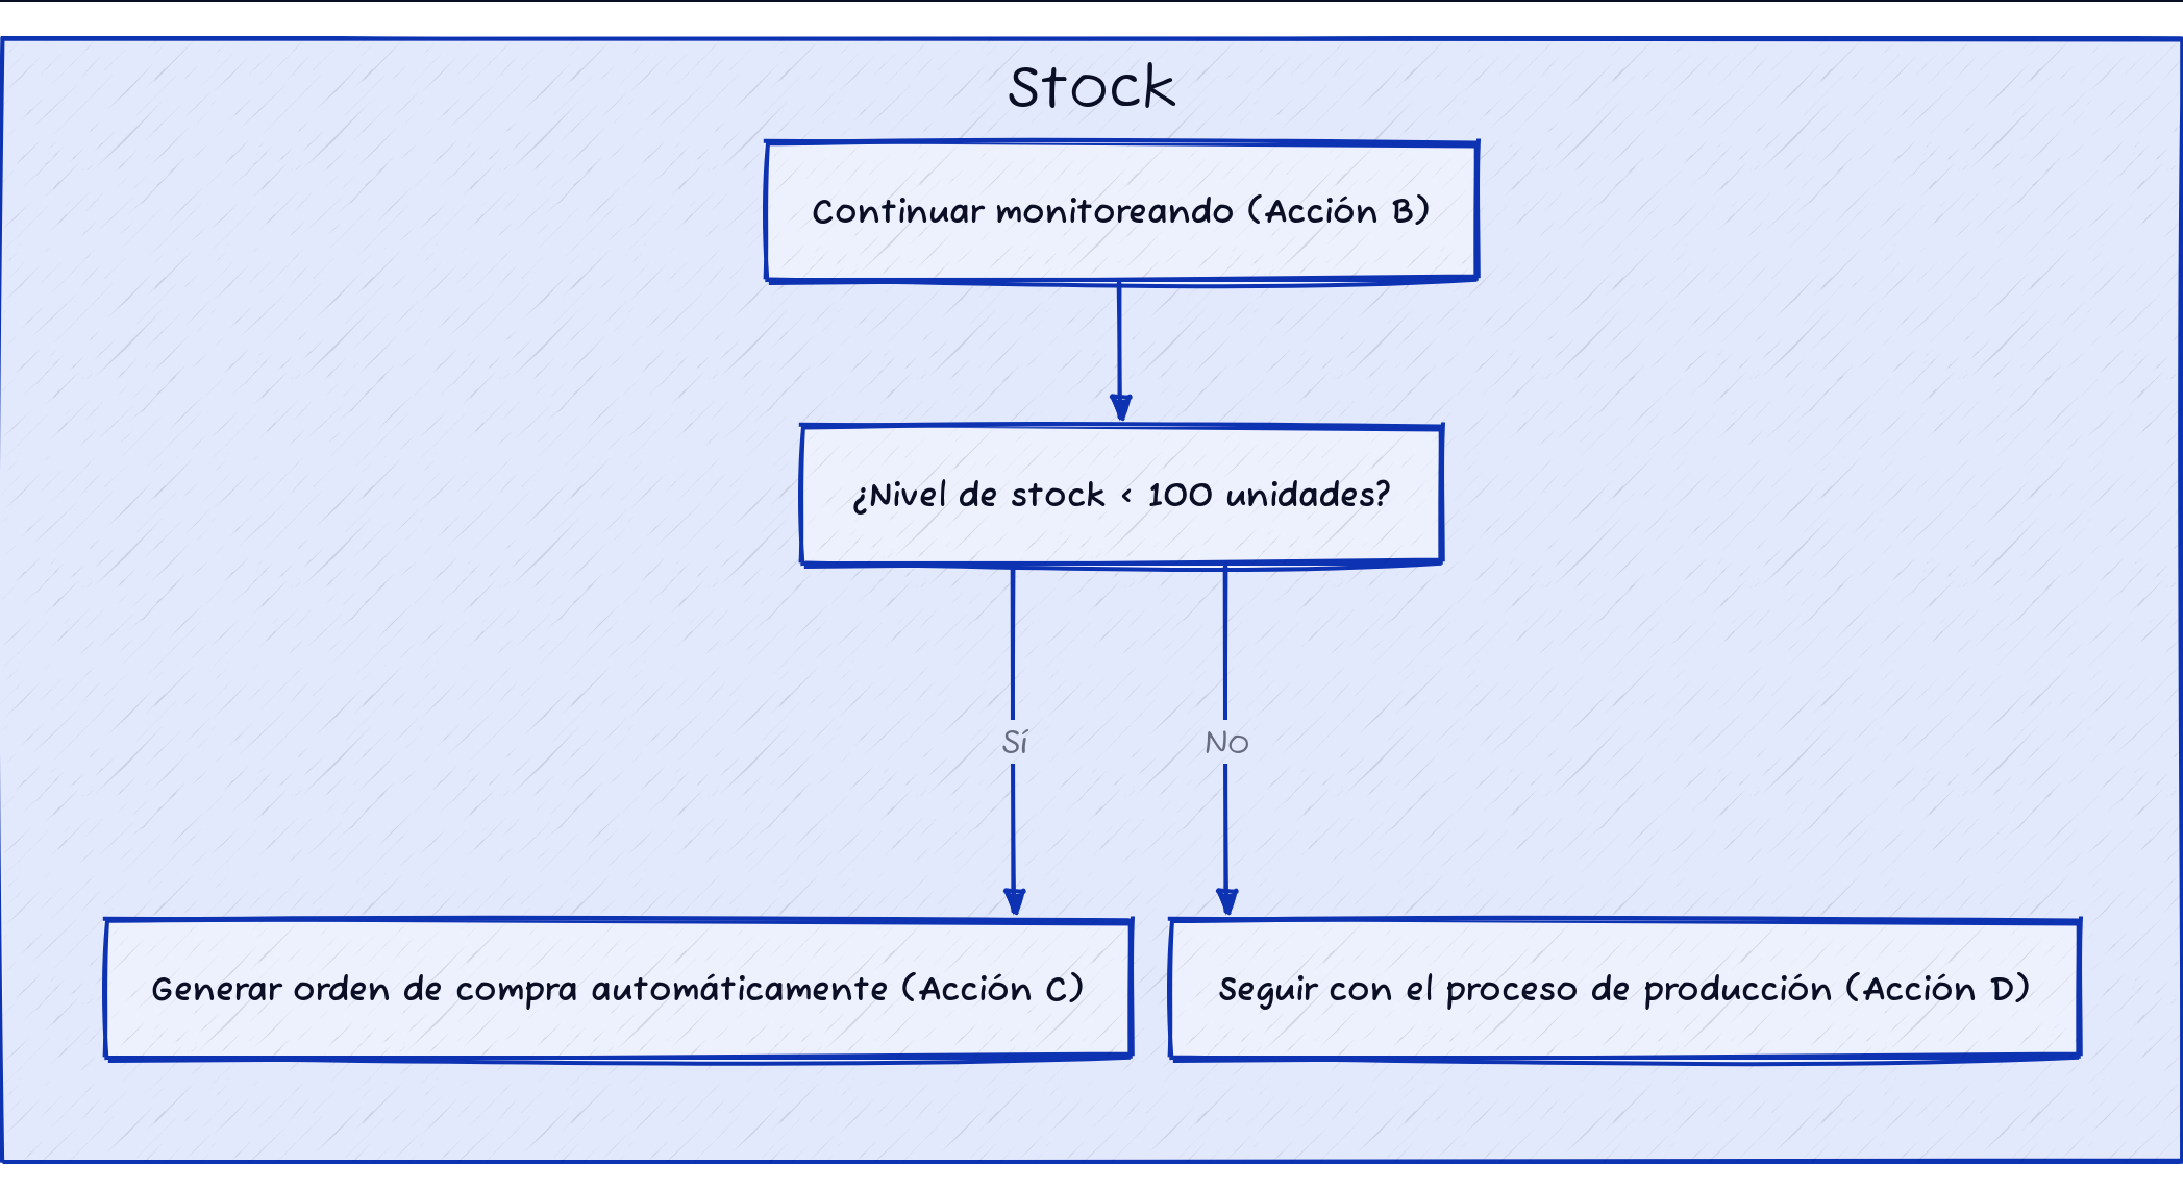
\includegraphics[h!,scale=0.5]{pdfs/diagram-2.pdf} 
\caption{Diagrama de flujo extendido para IA simbólica en un sistema de inventario}
\label{fig:diagrama-flujo-extendido}
\end{figure}

Este diagrama de flujo muestra un sistema de control de inventario más sofisticado que considera no solo los niveles de stock, sino también factores como el tiempo de entrega de los proveedores, la variabilidad de la demanda y los tiempos de producción.

\subsection{Conclusión: Primer Paso hacia la Automatización Inteligente}\label{conclusion}

La \textbf{IA Simbólica} es un paso esencial para que tu maquila avance hacia la automatización. Al establecer reglas claras y estructuradas, respaldadas por diagramas de flujo, puedes asegurar que todos los procesos se realicen de manera eficiente, sin depender de una sola persona o archivo.

Además, los sistemas basados en IA simbólica son ideales para procesos bien definidos y repetitivos, como el control de inventario y el mantenimiento preventivo. Si tu maquiladora aún depende de procesos manuales para gestionar el inventario o el mantenimiento, implementar IA simbólica te permitirá mejorar significativamente la eficiencia y reducir costos operativos.

\subsection{IA Simbólica: El Futuro del Control de Inventario}\label{futuro-ia-simbolica}

Al considerar el futuro del control de inventario en una maquiladora, la IA simbólica es solo el primer paso hacia una mayor automatización. Conforme avanza la tecnología, será posible integrar \textbf{Machine Learning} y \textbf{Big Data} para hacer que los sistemas no solo sigan reglas predefinidas, sino que también aprendan de los datos históricos y ajusten las reglas dinámicamente para optimizar aún más la eficiencia.

Por ejemplo, un sistema que combine IA simbólica con Machine Learning podría ajustar automáticamente los niveles mínimos de stock en función de la demanda estacional o las variaciones en los tiempos de entrega de los proveedores, optimizando continuamente el inventario sin necesidad de intervención humana.

\subsection{Implementación Práctica en el Contexto Actual}\label{implementacion-practica}

Hoy en día, muchas maquiladoras ya han comenzado a implementar sistemas basados en IA simbólica para la gestión del inventario, lo que ha reducido significativamente los tiempos de inactividad debido a la falta de materiales. Además, la reducción de errores humanos ha permitido a estas empresas operar de manera más eficiente y aumentar su productividad.

La implementación de sistemas de IA simbólica no requiere una infraestructura compleja. En muchos casos, se pueden integrar con los sistemas de ERP (Planificación de Recursos Empresariales) existentes, lo que facilita la transición hacia un modelo de producción más automatizado. 

Finalmente, una maquiladora que adopte IA simbólica y otras tecnologías relacionadas estará mejor preparada para enfrentar los retos de la industria 4.0, mejorando tanto su competitividad como su capacidad para responder rápidamente a las demandas del mercado.

